% This sample document was created by P.J. Healy (healy.52@osu.edu) for educational purposes. You may use this as a template for your own documents as you wish.

% Lines that start with a percent sign are just comments - they won't be processed or show up in the final output. If you actually want a percent sign to show up, use \% instead, like ``I got 100\%!''

% \documentclass says what type of document we're making and gives some basic options (options appear in square brackets. Here, our document is like an article (as opposed to a book, report, PhD thesis, etc.), we want 11-point font, and equation numbers on the left (leqno).
\documentclass[11pt,leqno]{article}

% These are the following packages we want LaTeX to load, since we might use them. I group them by similarity.
\usepackage{amsfonts,amsmath,amssymb,amsthm}
\usepackage{color,graphicx}
\usepackage{fullpage,setspace}
\usepackage[colorlinks=true,urlcolor=darkgray,bookmarks=false]{hyperref}

% First we tell LaTeX that we want to create a numbered "theorem-like" environment whose label is "Theorem X" and whose numbering will be handled by an internal counter named "theorem".
\newtheorem{theorem}{Theorem}
\newtheorem{example}{Example}

% The 'length variable' \parindent says how far to indent each paragraph. I want to set that length variable to zero:
\setlength{\parindent}{0mm}

% At OSU, you might use scarlet and gray colors for things, so here they are. Note: this requires the color package to be loaded. If you don't use this (and I don't below), you might as well comment it out or delete it.
\definecolor{scarlet}{cmyk}{0,1.00,0.65,0.15}
\definecolor{gray}{cmyk}{0.06,0,0,0.34}

\begin{document}


% First, move up from the normal starting point on the page by 20 millimeters so the table appears in the top margins
\vspace*{-20mm}

% Here's the actual table. We start with a `tabular' environment with 3 columns. The column alignments are left, center, and right, respectively, so the command option is {lcr}. Within the table, columns are delimited by & and rows by \\
% Note that LaTeX ignore consecutive spaces, including tabs, so you can use tabs to make your table look reasonable here.
\begin{tabular*}{\textwidth}{@{\extracolsep{\fill}}lcr}
Econ 8714     & \hfill    &         Professor: P.J. Healy          \\
Microeconomic Theory 2B  &           &   TA: Han Wang    
\end{tabular*}

% Finally, let's put a big `title' in the center of the page, after we `skip' down a bit of space.
\bigskip
\begin{center}
{\Large 03/03/2023 Recitation \#1 Handout}
\end{center}

% Skip some more space and then start working
\bigskip

\textbf{1. Pareto Optimality}
It is impossible to make anyone better-off without hurting someone. 

\textbf{2. Utility Possibility Set \& Utility Possibility Frontier}

 \begin{figure}[h]
    \centering
    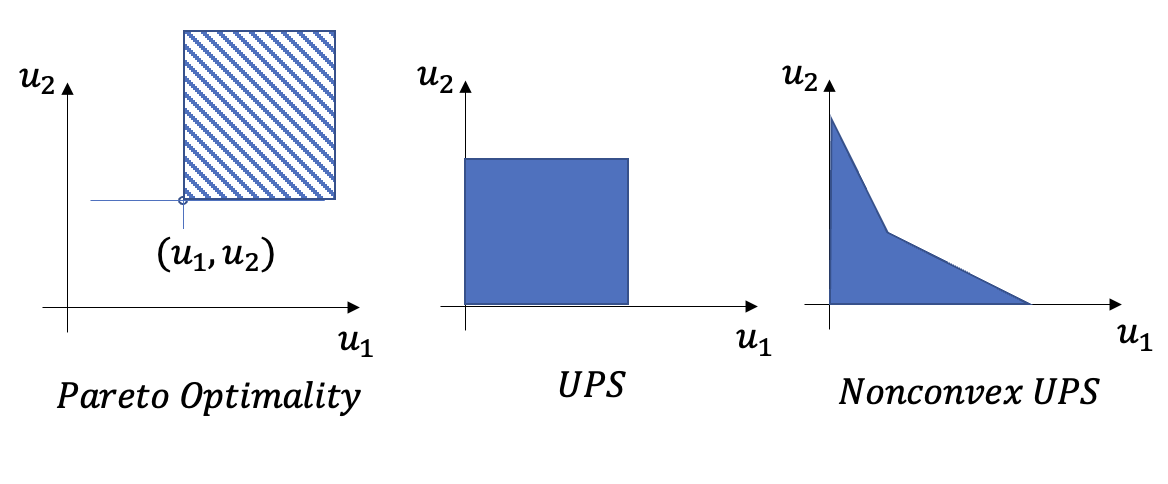
\includegraphics[width=0.5\textwidth]{figure 6.png}
    \caption{Pareto optimality, UPS \& UPF}
    \label{fig:3}
\end{figure}

We define UPF to be the set of utility vectors that correspond to Pareto optimal allocations.

Note: If UPS is a square, then UPF only contains a single point.

\textbf{3. Social Welfare Function}

A social welfare function aggregates individual preferences into social preferences. $W=F(u_{1},u_{2})$

 \begin{figure}[h]
    \centering
    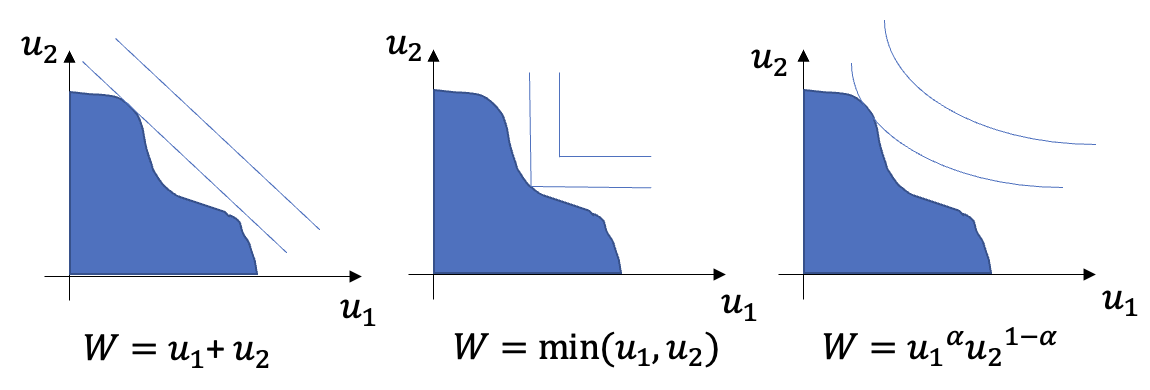
\includegraphics[width=0.5\textwidth]{figure 4.png}
    \caption{SWF}
    \label{fig:1}
\end{figure}

Question: Which SWF is reasonable?

%We want to find $F$ such that $z\in \arg\max_{z\in Z}F(u_{1}(z),u_{2}(z))$ implies that $z$ is Pareto optimal.
\begin{itemize}
    \item Convex UPS:  
    
    maximizing $\sum_{i}u_{i}$ can achieve ONE Pareto optimal allocation; 
    
    allowing for all possible weights ($\sum_{i}\lambda_{i}=1$ and $\lambda_{i}\geq 0$, $\forall i$) and maximizing $\sum_{i}\lambda_{i}u_{i}$ can achieve ALL Pareto optimal allocations. 

    (Intuition: supporting hyperplane theorem)
    \item Quasi-linear:  

    maximizing $\sum_{i}u_{i}$ can achieve ALL Pareto optimal allocations.  

    The following example shows that this statement is not true if we restrict allocations to be non-negative.
\end{itemize}

\begin{example}

$$
\begin{aligned}
& u_1\left(x_1, m_1\right)=\sqrt{x_1}+m_1 \\
& u_2\left(x_2, m_2\right)=\sqrt{x_2}+m_2 \\
& \left\{\left(\left(x_1, m_1\right),\left(x_2, m_2\right)\right) \in \mathbb{R}_{+}^2 \times \mathbb{R}_{+}^2: x_1+x_2=2, m_1+m_2=2\right\}
\end{aligned}
$$
Note that $a_1=\left(\left(x_1, m\right),\left(x_2, m_2\right)\right)=((2,2),(0,0))$ is P.O. 
This is the allocation where all resources go to agent 1. Clearly, giving more to agent 2 will hurt agent 1.
$a_2=((1,1),(1,1))$ yields the higher sum of $u_1$ and $u_2$.
\end{example}

 \begin{figure}[h]
    \centering
    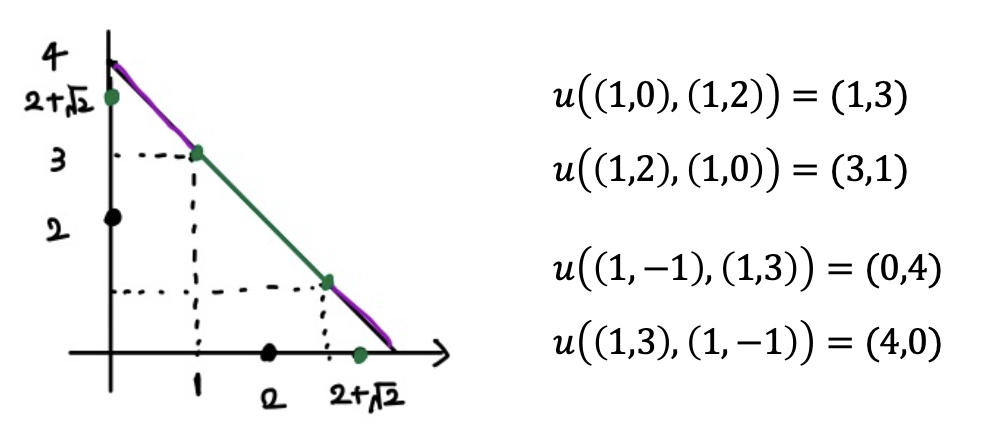
\includegraphics[width=0.5\textwidth]{figure 5.png}
    \caption{Maximizing $\sum_{i}u_{i}$ cannot achieve all P.O. allocations}
    \label{fig:2}
\end{figure}

\end{document} 